\documentclass[10pt,a4paper]{article}
\usepackage[latin1]{inputenc}
\usepackage[T1]{fontenc}
\usepackage{amsmath}
\usepackage{amsfonts}
\usepackage{amssymb}
\usepackage{graphicx}
\usepackage{hyperref}
\usepackage{amsthm}
\usepackage{tikz}
\usepackage{subcaption}
\usepackage[margin=2cm]{geometry}


\newtheorem{defn}{Definition}
\newtheorem{thm}{Theorem}


\author{Tobias Rohner}
\title{LehrFEM++ Hierarchic Finite Elements}


\begin{document}
    
\maketitle

\section{Polynomials}

    \begin{defn}
        Given $p \in \mathbb{N}$ and a polynomial $\psi(x) \in \mathcal{P}_p(\mathbb{R})$, we define the scaled polynomial $\psi(x;t)$ as
        \begin{equation*}
            \psi(x;t) := t^p\psi\left(\frac{x}{t}\right)
        \end{equation*}
    \end{defn}


\subsection{Shifted Legendre Polynomials}

    \begin{defn}[Shifted Legendre Polynomials]
        The Shifted Legendre Polynomials $P_n(\cdot;t) : [0, t] \to \mathbb{R}$ of degree $n \in \mathbb{N}$ are uniquely defined by the following properties:
        \begin{equation*}
            \int_0^1\! P_m(x;t)P_n(x;t) \,\mathrm{d}x = 0 \mbox{ if } m \neq n, \quad P_n(t;t) = 1
        \end{equation*}
    \end{defn}

    \begin{defn}[Integrated Shifted Legendre Polynomials]
        We define the Integrated Shifted Legendre Polynomials $L_n(\cdot;t) : [0, t] \to \mathbb{R}$ of degree $n \in \mathbb{N}$ as
        \begin{equation*}
            L_n(x;t) := \int_0^x\! P_{n-1}(\xi;t) \,\mathrm{d}x
        \end{equation*}
    \end{defn}
    
%    \begin{thm}
%        A recurrence relation for the \textit{Shifted Legendre Polynomials} $P_n(x;t) : [0,t] \to \mathbb{R}$ is given by
%        \begin{align*}
%            P_0(x;t) &= 1 \\
%            P_1(x;t) &= 2x - t \\
%            nP_n(x;t) &= (2n-1)(2x-t)P_{n-1}(x;t) - (n-1)t^2P_{n-2}(x;t) \mbox{ for } n \geq 2
%        \end{align*}
%    \end{thm}
%
%    \begin{thm}
%        A recurrence relation for the derivative of the \textit{Scaled Shifted Legendre Polynomials} $\partial_x P_n(x;t) : [0,t] \to \mathbb{R}$ is given by
%        \begin{align*}
%            \partial_x P_0(x;t) &= 0 \\
%            \partial_x P_n(x;t) &= 2nP_{n-1}(x;t) + (2x-t)\partial_xP_{n-1}(x;t) \mbox{ for } n \geq 1
%        \end{align*}
%    \end{thm}
%
%    \begin{thm}
%        A recurrence relation for the \textit{Integrated Shifted Legendre Polynomials} $L_n(\cdot;t) : [0, t] \to \mathbb{R}$ is given by
%        \begin{align*}
%            L_1(x;t) &= x \\
%            2(2n-1)L_n(x;t) &= P_n(x;t) - t^2P_{n-2}(x;t) \mbox{ for } n \geq 2
%        \end{align*}
%    \end{thm}
%
%    \begin{thm}
%        The derivative w.r.t. $x$ of the Integrated Shifted Legendre Polynomials is given by
%        \begin{equation*}
%            \partial_x L_n(x;t) = P_{n-1}(x;t)
%        \end{equation*}
%    \end{thm}
%
%    \begin{thm}
%        A recurrence relation of the derivative w.r.t. $t$ of the Integrated Shifted Legendre Polynomials is given by
%        \begin{align*}
%            \partial_t L_1(x;t) &= 0 \\
%            \partial_t L_n(x;t) &= -\frac{1}{2} \left( P_{n-1}(x;t) + tP_{n-2}(x;t) \right) \mbox{ for } n \geq 2
%        \end{align*}
%    \end{thm}
    
    
\subsection{Jacobi Polynomials}

    \begin{defn}[Jacobi Polynomials]
        The Jacobi Polynomials $\tilde{P}_n^{(\alpha,\beta)} : [-1, 1] \to \mathbb{R}$ of degree $n \in \mathbb{N}$ are uniquely defined by the following properties:
        \begin{equation*}
            \int_{-1}^1\! (1-x)^{\alpha}(1+x)^{\beta}\tilde{P}_n^{(\alpha,\beta)}(x)\tilde{P}_m^{(\alpha.\beta)}(x) \,\mathrm{d}x, \quad \tilde{P}_n^{(\alpha,\beta)}(1) = \binom{n+\alpha}{n}
        \end{equation*}
    \end{defn}

    \begin{defn}[Shifted Legendre Polynomials]
        We define the Shifted Legendre Polynomials $P_n^{(\alpha,\beta)} : [0, 1] \to \mathbb{R}$ of degree $n \in \mathbb{N}$ as
        \begin{equation*}
            P_n^{(\alpha,\beta)}(x) := \tilde{P}_n^{(\alpha,\beta)}(2x-1)
        \end{equation*}
    \end{defn}

    \begin{defn}[Integrated Shifted Legendre Polynomials]
        We define the Integrated Shifted Legendre Polynomials $L_n^{(\alpha,\beta)} : [0, 1] \to \mathbb{R}$ of degree $n \in \mathbb{N}$ as
        \begin{equation*}
            L_n^{(\alpha,\beta)}(x) := \int_0^x\! P_{n-1}^{(\alpha,\beta)}(x) \,\mathrm{d}x
        \end{equation*}
    \end{defn}

    For the sake of notational simplicity, we allow ourselves to ignore writing the $\beta$ parameter if it is equal to zero. We therefore have that
    \begin{equation*}
        P_n^{\alpha}(x) := P_n^{(\alpha,0)}(x), \quad L_n^{\alpha}(x) := L_n^{(\alpha,0)}(x)
    \end{equation*}


\section{Orientation Problems}

    \begin{figure}[ht!]
        \center
        \begin{subfigure}{0.45\textwidth}
            \center
            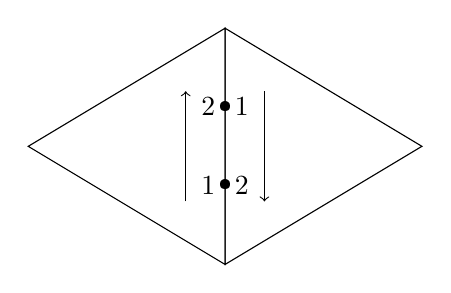
\begin{tikzpicture}
                % Draw the two triangles
                \draw[] (-2.5,0) -- (0,1.5) -- (0,-1.5) -- cycle;
                \draw[] (2.5,0) -- (0,-1.5) -- (0,1.5) -- cycle;
                % The orientation of the shared edge
                \draw[->] (-0.5,-0.7) -- (-0.5,0.7);
                \draw[->] (0.5,0.7) -- (0.5,-0.7);
                % Draw the conflicting DOF nodes on the shared edge
                \node at (0,0.5) {\textbullet};
                \node[anchor=west] at(0,0.5) {1};
                \node[anchor=east] at(0,0.5) {2};
                \node at (0,-0.5) {\textbullet};
                \node[anchor=west] at(0,-0.5) {2};
                \node[anchor=east] at(0,-0.5) {1};
            \end{tikzpicture}
        \end{subfigure}
        \begin{subfigure}{0.45\textwidth}
            \center
            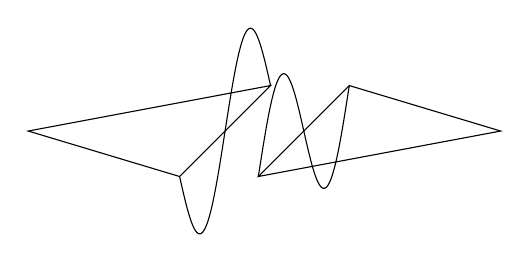
\begin{tikzpicture}
                % Draw the two triangles
                \draw[] (-3,0,0) -- (-0.5,0,1.5) -- (-0.5,0,-1.5) -- cycle;
                \draw[] (3,0,0) -- (0.5,0,-1.5) -- (0.5,0,1.5) -- cycle;
                % Draw the mismatched basis functions
                \draw[] (-0.5,0,-1.5)
                    \foreach \x in {1,...,100} {
                        -- (-0.5,{sin(3.6*\x)},{3*(\x-50)/100})
                    };
                \draw[] (0.5,0,-1.5)
                    \foreach \x in {1,...,100} {
                        -- (0.5,{sin(-3.6*\x)},{3*(\x-50)/100})
                    };
            \end{tikzpicture}
        \end{subfigure}
        \caption{Orientation Problem with Non-Lagrangian Finite Elements}
        \label{fig:orientation_problem}
    \end{figure}

    When using Lagrangian Finite Elements, we rely on the so called "glueing" in order to have a function space containing only continuous functions. This continuity is achieved by having a local numbering of DOFs as illustrated in \autoref{fig:orientation_problem} on the left. A single DOF may have different indices in the neighboring cells. Because the DOFs are symmetrically distributed on the edge, the two local basis functions of the neighboring cells will conveniently be continuous along the shared edge. However, if we do not use Lagrangian FEM, as is the case for Hierarchical FEM where the $n$-th edge DOF is the basis function coefficient for a polynomial of degree $n$, we no longer have continuity along the mesh edges (\autoref{fig:orientation_problem} on the right). In order to fix this, we must introduce a global ordering of the edge DOFs, as well as a global orientation of the edges. This is not a big problem though, as LehrFem++ mesh entities provide a function to access the global orientation of their edges. In the case the local orientation is flipped, we simply also flip the order of the local DOFs and the local coordinates at which we evaluate the edge basis functions. In the following sections, we will ignore this ordering problem and one simply has to apply the aforementioned transformations in order to obtain the basis on an arbitrary mesh entity.


\section{Basis Functions}

    We differentiate between three types of basis functions. The vertex basis functions, the edge basis functions and the face bubbles. The vertex basis functions will be nonzero on exactly one vertex and zero on all the others. The edge basis functions will be nonzero on an edge and zero on all other edges and the vertices. The face bubbles are nonzero only on the interior of the mesh entity while being zero on its boundary.


\subsection{Segment}

    \begin{figure}[ht!]
        \center
        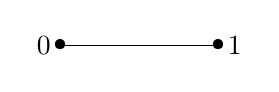
\begin{tikzpicture}
            % Edges
            \draw[] (0,0) -- (2,0);
            % Vertices
            \node at (0,0) {\textbullet};
            \node[anchor=east] at (0,0) {0};
            \node at (2,0) {\textbullet};
            \node[anchor=west] at (2,0) {1};
        \end{tikzpicture}
        \caption{Reference Element for the Segment}
        \label{fig:ref_segment}
    \end{figure}
    
    \begin{defn}[Vertex Basis Functions]
        We define the vertex basis functions of the segment as
        \begin{align*}
            \widehat{b_0^{\cdot}}(x) &:= 1 - x \\
            \widehat{b_1^{\cdot}}(x) &:= x
        \end{align*}
    \end{defn}

    \begin{defn}[Edge Basis Functions]
        We define the edge basis functions of the segment as
        \begin{equation*}
            \widehat{b_n^{-}}(x) := L_n(x) \mbox{ for } n \geq 2
        \end{equation*}
    \end{defn}


\subsection{Quadrilateral}

    \begin{figure}[ht!]
        \center
        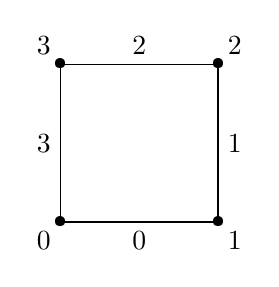
\begin{tikzpicture}
            % Edges
            \draw[] (0,0) -- (2,0) -- (2,2) -- (0,2) -- cycle;
            \node[anchor=north] at (1,0) {0};
            \node[anchor=west] at (2,1) {1};
            \node[anchor=south] at (1,2) {2};
            \node[anchor=east] at (0,1) {3};
            % Vertices
            \node at (0,0) {\textbullet};
            \node[anchor=north east] at (0,0) {0};
            \node at (2,0) {\textbullet};
            \node[anchor=north west] at (2,0) {1};
            \node at (2,2) {\textbullet};
            \node[anchor=south west] at (2,2) {2};
            \node at (0,2) {\textbullet};
            \node[anchor=south east] at (0,2) {3};
        \end{tikzpicture}
        \caption{Reference Element for the Quadrilateral}
        \label{fig:ref_quad}
    \end{figure}


\subsection{Triangle}


\section{Dual Basis}


\subsection{Segment}


\subsection{Quadrilateral}


\subsection{Triangle}
    
\end{document}